\documentclass[12pt,a4paper,titlepage,headinclude,bibtotoc]{scrartcl}

%---- Allgemeine Layout Einstellungen ------------------------------------------

% Für Kopf und Fußzeilen, siehe auch KOMA-Skript Doku
\usepackage[komastyle]{scrpage2}
\pagestyle{plain}
\setheadsepline{0.5pt}[\color{black}]
\automark[section]{chapter}
\usepackage{multirow}
\usepackage{caption}
\captionsetup{format=plain, font=footnotesize, labelfont= bf, width= 0.9\textwidth}
\captionsetup[table]{position=top}
%Einstellungen für Figuren- und Tabellenbeschriftungen
\setkomafont{captionlabel}{\sffamily\bfseries}
\setcapindent{0em}


%---- Weitere Pakete -----------------------------------------------------------
% Die Pakete sind alle in der TeX Live Distribution enthalten. Wichtige Adressen
% www.ctan.org, www.dante.de

% Sprachunterstützung
\usepackage[ngerman]{babel}

% Benutzung von Umlauten direkt im Text
% entweder "latin1" oder "utf8"
\usepackage[utf8]{inputenc}

% Pakete mit Mathesymbolen und zur Beseitigung von Schwächen der Mathe-Umgebung
\usepackage{latexsym,exscale,stmaryrd,amssymb,amsmath}


\usepackage[nointegrals]{wasysym}
\usepackage{eurosym}

% Anderes Literaturverzeichnisformat
%\usepackage[square,sort&compress]{natbib}
\usepackage{hyperref}
% Für Farbe
\usepackage{color}
\usepackage{graphicx}
\usepackage{wrapfig}
\usepackage{subfigure}

% Caption neben Abbildung
\usepackage{sidecap}


% Befehl für "Entspricht"-Zeichen
\newcommand{\corresponds}{\ensuremath{\mathrel{\widehat{=}}}}
% Befehl für Errorfunction
\newcommand{\erf}[1]{\text{ erf}\ensuremath{\left( #1 \right)}}


%Fußnoten zwingend auf diese Seite setzen
\interfootnotelinepenalty=1000

%Für chemische Formeln (von www.dante.de)
%% Anpassung an LaTeX(2e) von Bernd Raichle
\makeatletter
\DeclareRobustCommand{\chemical}[1]{%
  {\(\m@th
   \edef\resetfontdimens{\noexpand\)%
       \fontdimen16\textfont2=\the\fontdimen16\textfont2
       \fontdimen17\textfont2=\the\fontdimen17\textfont2\relax}%
   \fontdimen16\textfont2=2.7pt \fontdimen17\textfont2=2.7pt
   \mathrm{#1}%
   \resetfontdimens}}
\makeatother
\usepackage{textcomp}
\usepackage{upgreek}
%\begin{document}
%$\upmu$
%\end{document}
%Honecker-Kasten mit $$\shadowbox{$xxxx$}$$
\usepackage{fancybox}

%SI-Package
\usepackage{siunitx}

%keine Einrückung, wenn Latex doppelte Leerzeile
\parindent0pt

%Bibliography \bibliography{literatur} und \cite{gerthsen}
%\usepackage{cite}
\usepackage{babelbib}
\selectbiblanguage{ngerman}

\usepackage{siunitx}
%\begin{document}
 % \SI{1.55}{\micro\metre}
\sisetup{math-micro=\text{µ},text-micro=µ}
\usepackage{amsmath}

\usepackage[verbose]{placeins}
%für \FloatBarrier

\begin{document}

\begin{titlepage}
\centering
\textsc{\Large Physikalisch- Chemisches Grundpraktikum\\[1.5ex] Universität Göttingen}

\vspace*{0.5cm}

\rule{\textwidth}{1pt}\\[0.5cm]
{\huge \bfseries
  Versuch 2: \\[1.5ex]
Festkörperkette }\\[0.5cm]
\rule{\textwidth}{1pt}

\vspace*{0.5cm}


\begin{Large}
\begin{tabular}{ll}
Durchführende: &  Isaac Maksso, Julia Stachowiak\\
Assistent: & Sven Meyer \\
 Versuchsdatum: & 10.11.2016\\
 Datum der ersten Abgabe: & 17.11.2017\\
 Datum der zweiten Abgabe: & 1.12.2017\\
\end{tabular}
\end{Large}

\vspace*{0.5cm}


\begin{table}[h!]
\centering
\caption{Ergebnisse des Versuchs.}
\begin{tabular}{l|c|c}
Messgröße& Ergebniss&Literaturwert\\
\hline
$T_{\text{m}}^{\text{RECH}}$&379 ± 28\;K&\multirow{4}{*}{493.65\;K}\\
${T}_{\text{m}}^{\text{y-Ab}}$&476 ± 35\;K&\\
${T}_{\text{m}}^{\text{Vant}}$&492 ± 36\;K&\\
${T}_{\text{m}}^{\text{Graph}}$&471 ± 10\;K&\\
\end{tabular}
\end{table}
\end{titlepage}


\tableofcontents

\newpage


\section{Experimentelles}
\subsection{Experimenteller Aufbau}
\begin{figure}[h]
\centering
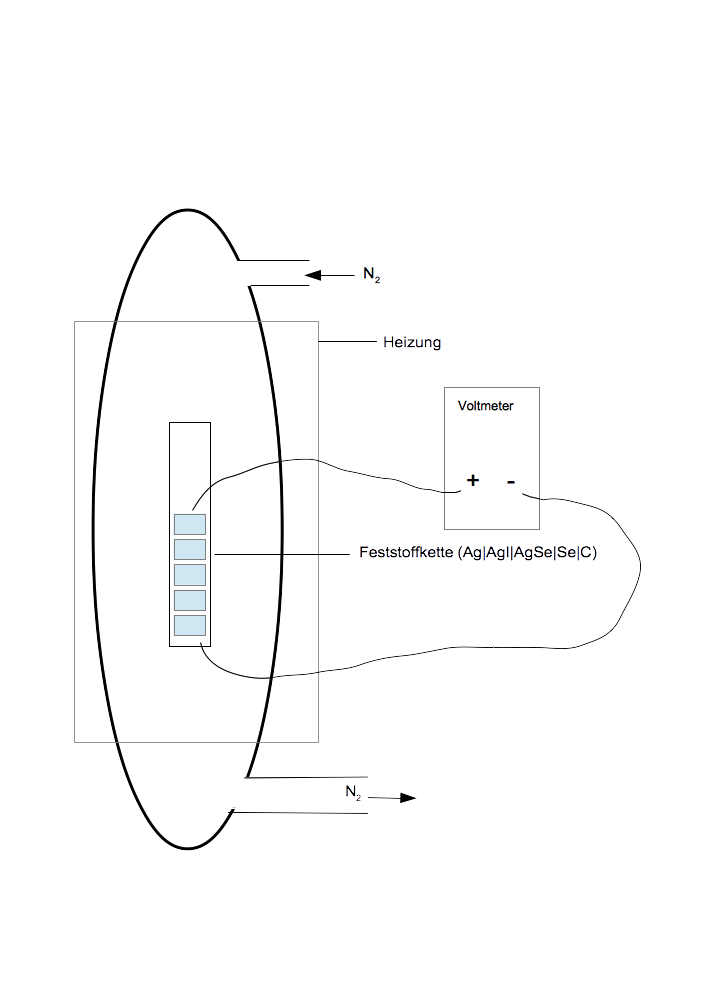
\includegraphics[width=9cm]{VB.png}
\caption{Der Versuchsaufbau sieht eine beheizte Feststoffkette unter Stickstoffatmossphäre vor. Die Festkörperfkette wurde in einem Magazin mit Platinelektroden aufgebaut und über Kabel an einem Voltmeter angeschlossen. Das Magazin wurde von einem Heizblock umschlossen.  Über das vom Heizblock umschlossene Magazin wurd eine Glasglocke übergestülpt, wo die Stickstoffatmosphäre eingestellt wird.}
\end{figure} 
\FloatBarrier
\subsection{Durchführung}
Es wurde 0.4002\;g Silberiodid abgewogen und zu einer Tablette gepresst. Es wurde eine Festkörperkette, wie in Abbildung 1 zu sehen ist, aufgebaut und 10\;min mit $\text{N}_2$-Gas umspült. Die Feststoffkette wurde auf 160\;°C hochgeheizt und 45\;min bei einem Strom von 1.2\;mA aufgeladen. Es wurde ab 160\;°C in 5\;°C-Schritten die Spannung gemessen. Ab 175\;°C wurde das Messgerät einmalig kurzgeschlossen und die Messung fortgesetzt. 
\section{Auswertung}
\subsection{Messergebnisse}
In der Tabelle 2 sind die Messergebnisse der Elektromotorischenkraft dargestellt.
\begin{table}[h!]
\centering
\caption{Messergebnisse des Versuchs.}
\begin{tabular}{c|c||c|c}
T/\;K & EMK/\;V &T/\;K & EMK/\;V\\ 
\hline
433.7 & 0.2889 &   488.15 &0.2860\\ 
438.5 & 0.2871 & 493.15&0.2868 \\
443.25 & 0.2772 &  498.15&0.2877\\
448.15 & 0.2782 & 503.15& 0.2885\\
453.15 &0.2792 & 508.15 &0.2893\\
458.15 & 0.2803 & 513.15 &0.2900\\
463.15 &0.2814 & 518.15 &0.2903\\
468.15 &0.2826 & 523.15&0.2916\\
473.15 &0.2838 & 528.15 & 0.2923\\
478.15 & 0.2844 & 533.15& 0.2933\\
483.15 & 0.2852 &&\\
\end{tabular} 
\end{table}
\FloatBarrier
\subsection{Auftragung von $\Delta_\text{R} G$($T$) gegen $T$}
Die freie Reaktionsenergie $\Delta_\text{R} G$ lässt sich nach Gl.\;1 errechnen:
\begin{align}
\Delta_\text{R} G &= - z F \Delta E 
\end{align}
$\Delta E$ berechnet sich folgendermaßen:
\begin{align}
\Delta E &= \Delta E^0 + z\cdot F \cdot \frac{\text{a}(\text{Ag}_2\text{Se})}{\text{a}(\text{Ag})^2\cdot\text{a}(\text{Se})}\\
\Delta E &= \Delta E^0 + R\cdot T\cdot \text{ln}(\frac{1}{1^2\cdot1})\\
\Delta E &= \Delta E^0 + R\cdot T \cdot \text{ln}(1)\\
\Delta E &= \Delta E^0 \\
\end{align}
Da die Aktivität von Feststoffen 1 ist, fällt der logorithmische Term weg und Die EMK ist gleich dem Standardelektrodenpotential.\\
Die Werte für $\Delta_\text{R} G$ ($T$) sind in der Tabelle\;3 dargestellt.
\begin{table}[h!]
\centering
\caption{Ergebnisse für $\Delta_\text{R} G$.}
\begin{tabular}{c|c||c|c}
$T$/\;K & $\Delta_\text{R} G$/\;$\frac{\text{kJ}}{\text{mol}}$ &$T$/\;K & $\Delta_\text{R} G$/\;$\frac{\text{kJ}}{\text{mol}}$\\ 
\hline
433.7 & -55.75 &488.15 & -55.19 \\ 
438.5 & -57.33 & 493.15& -55.52 \\
443.25 & -55.42 &  498.15& -55.67\\
448.15 & -53.68 & 503.15&  -55.83\\
453.15 & -53.88 & 508.15 & -55.96\\
458.15 & -54.09 & 513.15 & -56.12\\
463.15 & -54.30 & 518.15 & -56.12\\
468.15 & -54.53 & 523.15& -56.27\\
473.15 & -54.77 & 528.15 & -56.41\\
478.15 & -54.88 & 533.15& -56.60\\
483.15 & -55.04 &&\\
\end{tabular} 
\end{table}
\FloatBarrier
Der Fehler der freien Reaktionsenthalpie $\Delta(\Delta_\text{R} G)$  wird mittels Fehlerfortpflanzung berechnet. Bei den ersten drei Messungen schwankte die Anzeige auf dem Voltmeter. Es wurde die Schwankung als Fehler notiert. Ab der vierten Messung konnte die EMK ohne Schwankungen abgelesen werden. Der Fehler wird auf 0,0005\;V geschätzt:
\begin{align}
\Delta(\Delta_R G)= \sqrt{(-z\cdot F \cdot \Delta(\Delta E))^2}
\end{align}
\begin{table}[h]
\centering
\caption{Fehler für $\Delta_\text{R} G$.}
\begin{tabular}{c|c|c}
$T$/ K & $\Delta(\Delta E)$/ V & $\Delta(\Delta_\text{R} G)$/\;$\frac{\text{kJ}}{\text{mol}}$ \\
\hline
433.7 &  0.005 &  0.1  \\
438.5 & 0.003   & 0.06 \\
443.25 & 0.003  & 0.06 \\
448.15 &  0.0005& 0.01 \\
453.15 & 0.0005& 0.01 \\
458.15 &  0.0005& 0.01 \\
463.15 & 0.0005& 0.01 \\
468.15 & 0.0005& 0.01 \\
473.15 & 0.0005& 0.01 \\
478.15 & 0.0005& 0.01 \\
483.15 & 0.0005& 0.01 \\
488.15 & 0.0005& 0.01 \\
493.15 & 0.0005& 0.01 \\
498.15 & 0.0005& 0.01 \\
503.15 & 0.0005& 0.01 \\
508.15 & 0.0005& 0.01 \\
513.15 & 0.0005& 0.01 \\
518.15 & 0.0005& 0.01 \\
523.15 & 0.0005& 0.01 \\
528.15 & 0.0005& 0.01 \\
533.15 & 0.0005& 0.01 \\
\end{tabular}
\end{table}
\FloatBarrier
\subsection{Auftragung von $\Delta E$ gegen $T$}
Es wurden die Werte für $\Delta E$ und $T$ aus Tabelle\;2 mit den Fehlern aus für $\Delta E$ aus Tabelle\;3 aufgetragen in Abbildung\;2 aufgetragen. Die Temperatur wurde als fehlerfrei angenommen, da diese nach einer langen Aufheizphase durch kleine Temperaturerhöhungen mittels Temperatursteuerung eingestellt wurde. Es wurden bei der linearen Regression die ersten drei Messpunkte nicht eingefügt, da sie sehr stark von den folgenden Messwerten abweichen. 
\begin{figure}[h]
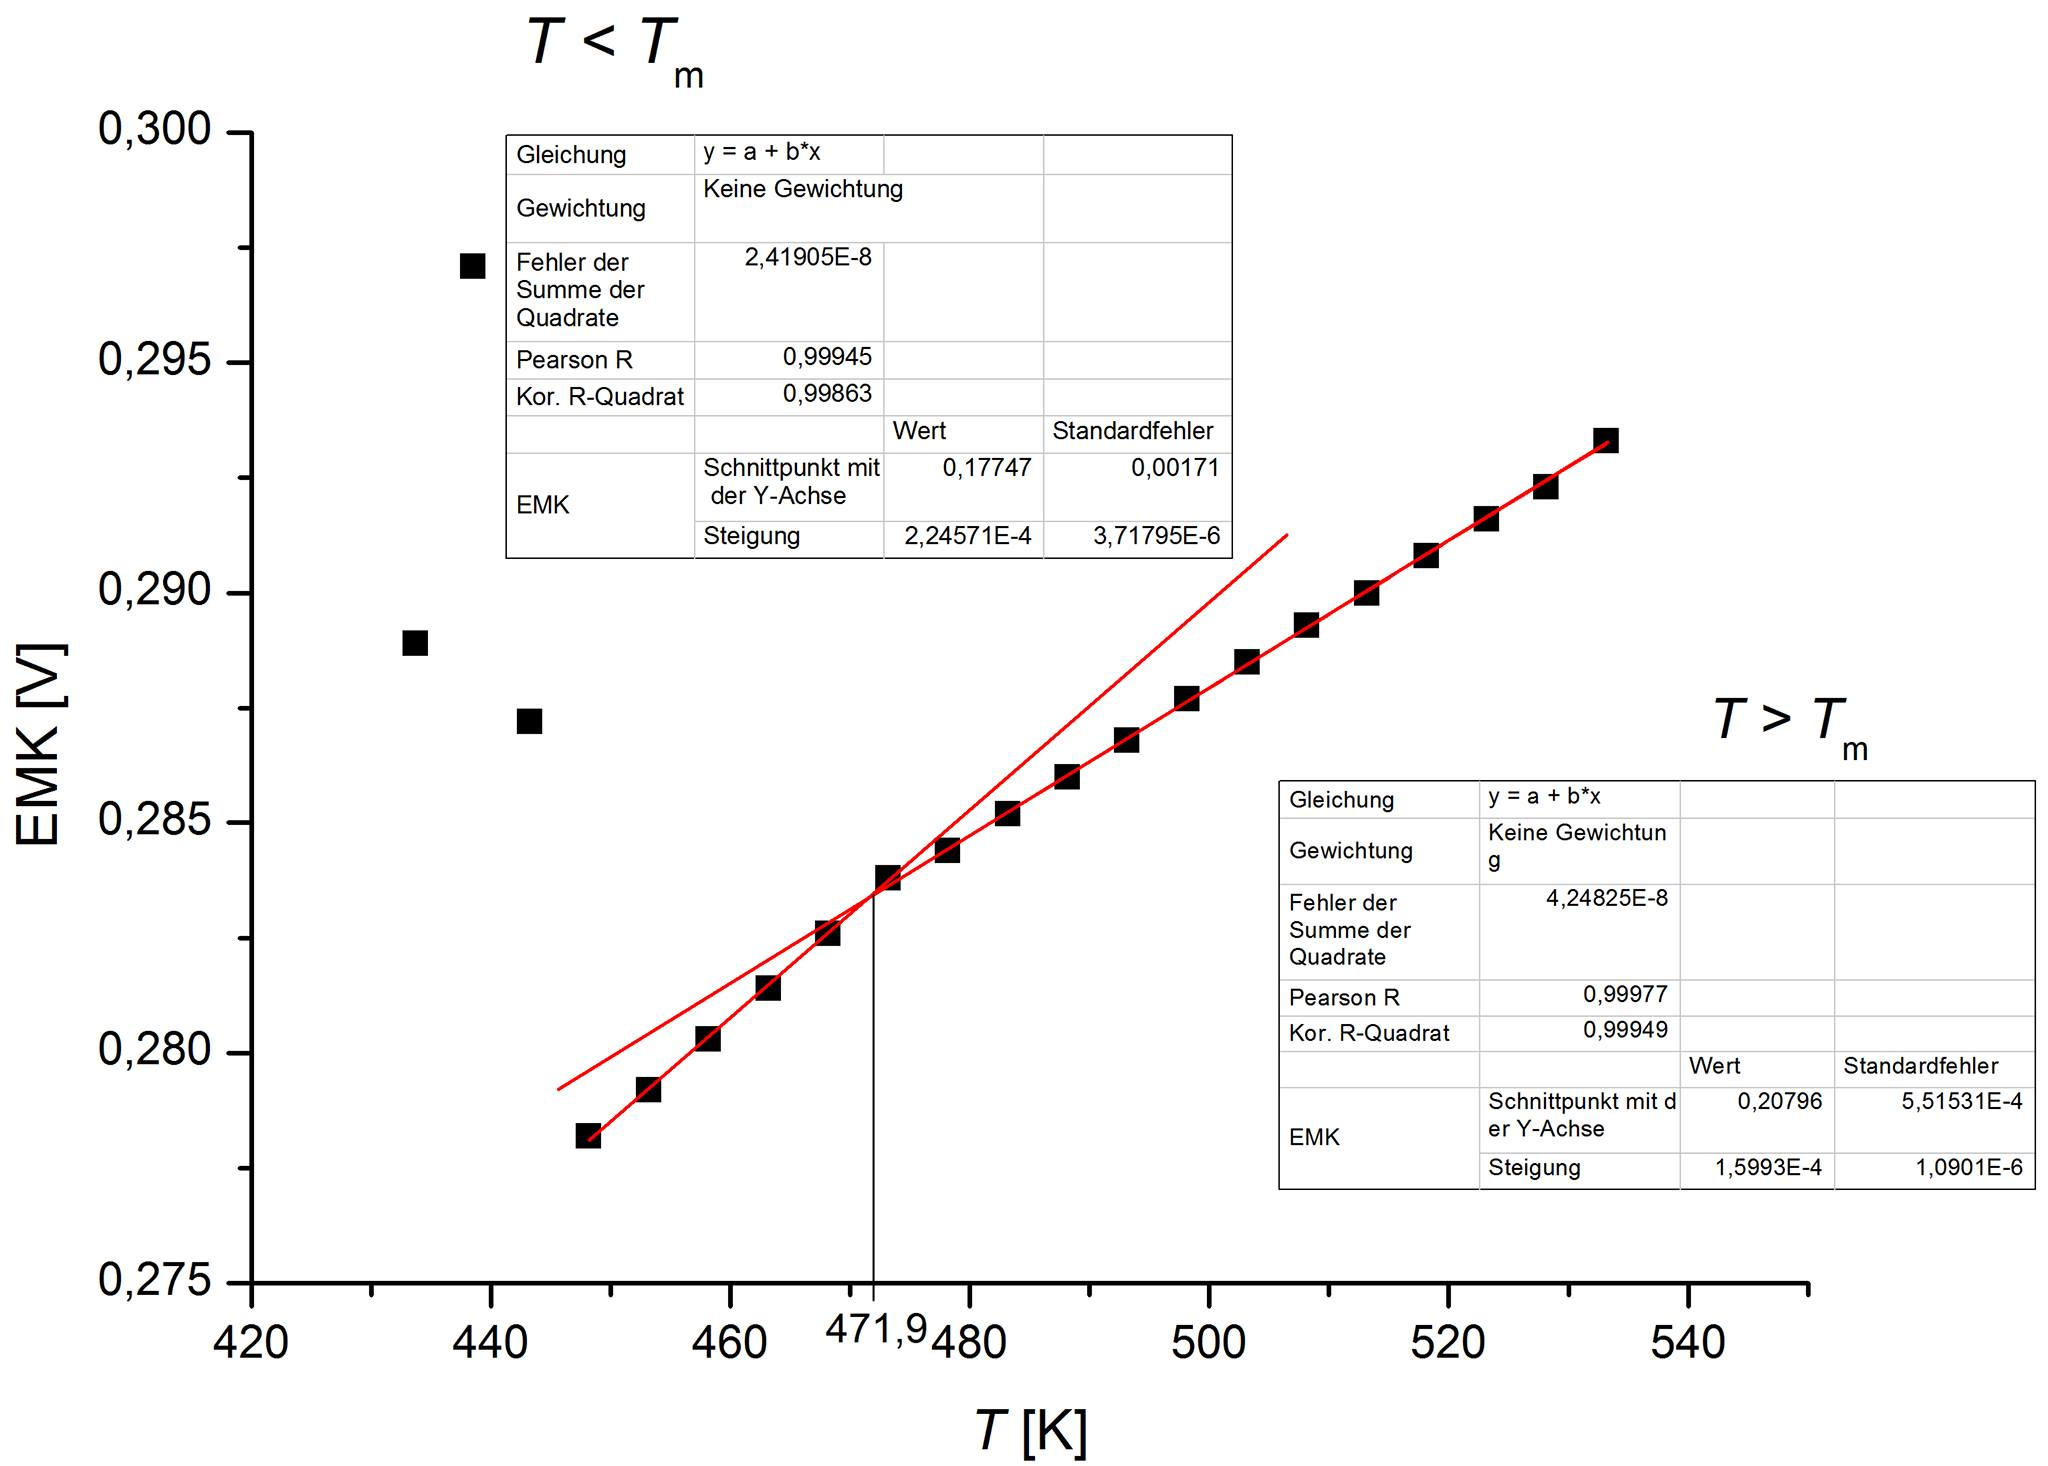
\includegraphics[width=13.5cm]{EGT.jpeg}
\caption{Auftragung von $\Delta E$ gegen T.}
\end{figure} 
\FloatBarrier
Die negative Ableitung der freien Reaktionsentalpie nach der Temperatur ist gleich der Reaktionsentropie (Siehe Gleichung\;8). Durch einsetzen der Gleichung~1 wird die Formel zur Berechnung der Reaktionsentropie erhalten. 
\begin{align}
\Delta_\text{R} S &= -\left(\frac{\partial \Delta_R G}{\partial T}\right)\\
&= z \cdot F \cdot \left(\frac{\partial \Delta E}{\partial T}\right)\\
&= z \cdot F \cdot m \\
\Delta_\text{R} S_{\text{s}} &= 2 \cdot 9.6485 \cdot 10^4\;\text{As} \cdot 2.24 \cdot 10^{-4}\;\frac{\text{J}}{\text{K}\cdot\text{mol}}\\
&= 43.3\;\frac{\text{J}}{\text{K}\cdot\text{mol}}\\
\Delta_\text{R}  S_{\text{l}} &= 2 \cdot  9.6485 \cdot 10^4\;\text{As} \cdot 1.60 \cdot 10^{-4}\;\frac{\text{J}}{\text{K}\cdot\text{mol}}  \\
&= 30.9\;\frac{\text{J}}{\text{K}\cdot\text{mol}}
\end{align}
Der Fehler der Reaktionsentropie lässt sich mittels Fehlerfortpflanzung berechnen. Der Fehler der Steigung wird hierbei von Origin entnommen. 
\begin{align}
\Delta(\Delta_\text{R}  S)&= \sqrt{(z\cdot F \cdot \Delta m)^2}\\
\Delta(\Delta_\text{R}  S_{\text{s}})&= \sqrt{\left(2\cdot 9.6485 \cdot 10^4\;\text{As} \cdot 0.04 \cdot 10^{-4}\;\frac{\text{J}}{\text{K}\cdot\text{mol}}\right)^2}\\
&= 0.7 \;\frac{\text{J}}{\text{K}\cdot\text{mol}}\\
\Delta(\Delta_\text{R}  S_{\text{l}})&= \sqrt{\left(2\cdot 9.6485 \cdot 10^4\;\text{As} \cdot 0.01\cdot 10^{-4}\;\frac{\text{J}}{\text{K}\cdot\text{mol}}\right)^2}\\
&= 0.2\;\frac{\text{J}}{\text{K}\cdot\text{mol}}
\end{align}
\subsection{Bestimmung der Reaktionsenthalpie}
Aus der Gibbs-Helmholtz-Gleichung ergibt sich die Reaktionsentalpie:
\begin{align}
\Delta_\text{R} H=& \Delta_\text{R} G +{T} \cdot \Delta_\text{R} S
\end{align}
Der Fehler lässt sich durch die Fehlerfortpflanzung ermitteln. Es wurde für $\Delta(\Delta_\text{R} G)$ die Werte aus Tabelle\;4 und für $\Delta(\Delta_\text{R} S)$ die Fehler aus Gl.\;12 oder 14 benutzt:
\begin{align}
\Delta(\Delta_\text{R}  H)&= \sqrt{(\Delta(\Delta_\text{R} G))^2 + (\Delta(\Delta_\text{R} S) \cdot {T})^2 +(\Delta {T} \Delta_\text{R} S)^2}\\
\end{align}
\begin{table}[h]
\centering
\caption{Fehler für $\Delta_\text{R} G$.}
\begin{tabular}{c|c|c}
$T$/ K &Aggregatzustand&$\Delta_\text{R} H$/ \;$\frac{\text{kJ}}{\text{mol}}$ \\
\hline
433.7 ± 0.05 & \multirow{7}{*}{s.} & -37.0 ± 1.0\\
438.5 ± 0.05   &  & -38.3 ± 0.7 \\
443.25 ± 0.1  &  & -36.2 ± 0.7\\
448.15 ± 0.05&  &-34.3 ± 0.3\\
453.15 ± 0.05&  &-34.2 ± 0.3\\
458.15 ± 0.05&  &-34.2 ± 0.3\\
463.15 ± 0.05&  &-34.2 ± 0.3\\
468.15 ± 0.05&  &-34.2 ± 0.3\\
\hline
473.15 ± 0.05& \multirow{12}{*}{l.} &-40.2 ± 0.1\\
478.15 ± 0.05&  &-40.1 ± 0.1\\
483.15 ± 0.05&  &-40.1 ± 0.1\\
488.15 ± 0.05&  &-40.1 ± 0.1\\
493.15 ± 0.05&  &-40.3 ± 0.1\\
498.15 ± 0.05&  &-40.3 ± 0.1\\
503.15 ± 0.05&  &-40.3 ± 0.1\\
508.15 ± 0.05&  &-40.3 ± 0.1\\
513.15 ± 0.05&  &-40.3 ± 0.1\\
518.15 ± 0.05&  &-40.1 ± 0.1\\
523.15 ± 0.05&  &-40.1 ± 0.1\\
528.15 ± 0.05&  &-40.1 ± 0.1\\
533.15 ± 0.05&  &-40.1 ± 0.1\\
\end{tabular}
\end{table}
\FloatBarrier
Die Werte sind von 433.7\;K bis 468.15\;K und 473.15\;K bis 533.15\;K nahezu konstant. Es wird aufgrunddessen der Mittelwert gebildet, um die Reaktionsenthalpie der festen beziehungsweise flüssigen Phase zu bestimmen. Der Fehler wird gemittelet:
\begin{align}
\Delta_\text{R} H_{\text{x}}&= \frac{1}{n}  \sum_{n=i}^i \Delta_\text{R} H_i  \\
\Delta_\text{R} H_{\text{s}}^{\text{RECH}}&= -35.3 \pm 0.5\;\frac{\text{kJ}}{\text{mol}}\\
\Delta_\text{R} H_{\text{l}}^{\text{RECH}}&= -40.2 \pm 0.2\;\frac{\text{kJ}}{\text{mol}}
\end{align}
Es ist möglich die Reaktionsenthalpie aus der Auftragung EMK gegen T zu bestimmen. Hierbei erden die Ausdrück für die freie Reaktionsenthalpie und Reaktionsentropie aus der Gleichung\;20 durch die Ausdrücke aus Gleichung\;9 und 1 ersetzt:
\begin{align}
\Delta_\text{R} H=&  - z\cdot F \cdot\Delta E +  z \cdot F \cdot \left(\frac{\partial \Delta E}{\partial T}\right)\cdot\text{T} \\ 
\Delta_\text{R} H(0)=&  - z\cdot F\cdot \Delta E(0) +  z \cdot F \cdot \left(\frac{\partial \Delta E}{\partial T}\right)\cdot 0\\ 
\Delta_\text{R} H(0)=&  - z\cdot F \cdot\Delta E(0)
\end{align}
Die Werte für $\Delta E(0)$ wurde aus der Auftragung\;1 abgelesen. 
\begin{align}
\Delta_\text{R} H_{\text{s}}^{\text{y-Ab}}=& -34.2\;\frac{\text{kJ}}{\text{mol}}\\
\Delta_\text{R} H_{\text{l}}^{\text{y-Ab}}=&  -40.1\;\frac{\text{kJ}}{\text{mol}}
\end{align}
Der Fehler wurde mittels Fehlerfortpflanzung bestimmt. Der Fehler des y-Achsenabschnitts wurde aus dem Analysedataenblatt des Zeichenprogramms entnommen.
\begin{align}
\Delta(\Delta_\text{R} H)=& \sqrt{(- z\cdot F \cdot\Delta(\Delta E(0)))^2}\\
\Delta(\Delta_\text{R} H_{\text{s}}^{\text{y-Ab}})&  0.4\;\frac{\text{kJ}}{\text{mol}}\\
\Delta(\Delta_\text{R} H_{\text{l}}^{\text{y-Ab}})=&  0.1\;\frac{\text{kJ}}{\text{mol}}
\end{align}
\subsection{Auftragung nach Vant'Hoff}
Zwischen der Gleichgewichtskonstante und der freien Reaktionsenthalpie besteht folgender Zusammenhang:
\begin{align}
\text{K}&=e^{-\frac{\Delta_\text{R} G}{RT}}
\end{align}
In Gl.\;28 wird Gl.\;1 eingesetzt und der natürliche Logorithmus gezogen:
\begin{align}
\text{K}&=e^{-\frac{zF\Delta E}{RT}}\\
\text{ln(K)}&=-\frac{zF\Delta E}{RT}
\end{align}
Die Reaktionsenthalpie kann durch die Vant'Hoff Gleichung aus der Steigung ermittelt werden. Die Wert der aufgetragenen Punkte sind in Tabelle\;6 aufgelistet. Die Steigung wurde aus der Abbildung\;3 abgelesen
\begin{align}
\Bigl(\frac{\partial\text{ln}(K)}{\partial{T}^{-1}}\Bigr)_p&=\frac{-\Delta_R H}{R}\\
\Delta_\text{R} H&=- \Bigl(\frac{\partial\text{ln}(K)}{\partial {T}^{-1}}\Bigr)_p\cdot R\\
\Delta_\text{R} H&=- m_x\cdot R\\
\Delta_\text{R} H_{\text{s}}^{\text{Vant}}&=-40.4\;\frac{\text{kJ}}{\text{mol}}\\
\Delta_\text{R} H_{\text{l}}^{\text{Vant}}&=-34.3\;\frac{\text{kJ}}{\text{mol}}\\
\end{align}
\begin{table}[h]
\centering
\caption{Wert für die Auftragung nach Van't Hoff.}
\begin{tabular}{c|c|c}
${T}^{-1}$/ $10^{-3}\text{K}^{-1}$ &Aggregatzustand& ln($K$) \\
\hline
2.31 &  \multirow{7}{*}{s.} & 15.5\\
2.28 & & 15.7 \\
2.26 & &15.0\\
2.23 & &14.4\\
2.21 & &14.3\\
2.18 &&14.2\\
2.16 &  &14.1\\
2.14 &  &14.0\\
\hline
2.11 & \multirow{12}{*}{l.} &13.9\\
2.10 &  &13.8\\
2.07 &  &13.7\\
2.05  &  &13.6\\
2.03 &  &13.5\\
2.01 &  &13.4\\
1.99 &  &13.3\\
1.97 &  &13.2\\
1.95 &  &13.2\\
1.93 &  &13.0\\
1.91 &  &12.9\\
1.89 &  &12.8\\
1.88 &  &12.8\\
\end{tabular}
\end{table}
\FloatBarrier
\begin{figure}[h]
\includegraphics[width=13.5cm]{Vant.jpeg}
\caption{Auftragung nach Van't Hoff.}
\end{figure} 
\FloatBarrier
Der Fehler der Reaktionsenthalpie lässt sich mittels Fehlerfortpflanzung ermitteln. Der Fehler der Steigung wurde aus aus dem Analysdatenblatt der Auftragung entnommen:
\begin{align}
\Delta(\Delta_\text{R} H) &= \sqrt{(R\cdot\Delta m)^2}\\
\Delta(\Delta_\text{R} H_{\text{s}}) &= 0.8\;\frac{\text{kJ}}{\text{mol}}\\
\Delta(\Delta_\text{R} H_{\text{l}}) &= 0.4\;\frac{\text{kJ}}{\text{mol}}
\end{align}
\subsection{Bestimmung der Umwandlungsenthalpie und Umwandlungsentropie}
Die Umwandungsenthalpie wird aus der Differenz zwischen der Reaktionsenthalpie der festen und der flüssigen Phase bestimmt. Hierbei wird die Unwandlungsenthalpie aus dem Mittelwert der rechenerischen Werte aus Tabelle\;5 ($\Delta_\text{U} H_{\text{s}\rightarrow\text{l}}^{\text{RECH}}$) und die Umwandlungsenthalpie aus den y-Abschnitten-Rechnungen Gl.\;26 und 27 ($\Delta_\text{U} H_{\text{s}\rightarrow\text{l}}^{\text{y-Ab}}$) berechnet. Der Fehler wurde durch die Summe der Fehler der Reaktionenthalpie in der flüssigen und festen Phase bestimmt:
\begin{align}
\Delta_\text{U} H_{\text{s}\rightarrow\text{l}}^{\text{RECH}}=&  -40.2\;\frac{\text{kJ}}{\text{mol}} - \Bigl(-35.3\;\frac{\text{kJ}}{\text{mol}}\Bigr) \pm \Bigl((0.2+0.5)\;\frac{\text{kJ}}{\text{mol}}\Bigr)\\
\Delta_\text{U} H_{\text{s}\rightarrow\text{l}}^{\text{RECH}}=& -4.7\pm 0.7 \;\frac{\text{kJ}}{\text{mol}}\\
\Delta_\text{U} H_{\text{s}\rightarrow\text{l}}^{\text{y-Ab}}=&  -40.1\;\frac{\text{kJ}}{\text{mol}} - \Bigl(-34.2\;\frac{\text{kJ}}{\text{mol}}\Bigr) \pm \Bigl((0.4+0.1)\;\frac{\text{kJ}}{\text{mol}}\Bigr)\\
\Delta_\text{U} H_{\text{s}\rightarrow\text{l}}^{\text{y-Ab}}=& -5.9 \pm 0.5 \;\frac{\text{kJ}}{\text{mol}}\\
\Delta_\text{U} H_{\text{s}\rightarrow\text{l}}^{\text{Vant}}=&  -40.4\;\frac{\text{kJ}}{\text{mol}} - \Bigl(-34.3\;\frac{\text{kJ}}{\text{mol}}\Bigr) \pm \Bigl((0.8+0.4)\;\frac{\text{kJ}}{\text{mol}}\Bigr)\\
\Delta_\text{U} H_{\text{s}\rightarrow\text{l}}^{\text{Vant}}=& -6.1 \pm 1.2 \;\frac{\text{kJ}}{\text{mol}}
\end{align}
Die Umwandlungsentropie berechnet sich ähnlich der Umwandlungsenthalpie aus der Different der Reaktionsentropien der festen und flüssigen Phase. Die Fehler wurden zu Größtfehlern summiert. Es wurden die Werte aus den Gleichungen\;12, 14, 17 und 19 genutzt:
\begin{align}
\Delta_\text{U} S_{\text{s}\rightarrow\text{l}}=&  30.9\;\frac{\text{J}}{\text{K}\cdot\text{mol}} - 43.3\;\frac{\text{J}}{\text{K}\cdot\text{mol}} \pm \Bigl((0.7+0.2)\;\frac{\text{J}}{\text{K}\cdot\text{mol}}\Bigr)\\
\Delta_\text{U} S_{\text{s}\rightarrow\text{l}}=& -12.4\pm0.9 \;\frac{\text{J}}{\text{K}\cdot\text{mol}}
\end{align}
\subsection{Schmelzpunktbestimmung}
Ist das System im Phasengleichgewicht, ist die freie Reaktionsenthalpie gleich 0. Die Gibbs-Hemlholzgleichung (Gl.\;20) wird kann nach $T$ umgestellt werden. Um die Schmelztemperatur bestimmen zu können wird der Quotient aus der Umwandlungsenthalpie und der Umwandlungsentropie aufgestellt:
\begin{align}
{T}_{\text{m}}= \frac{\Delta_\text{U} H_{\text{s}\rightarrow\text{l}}}{\Delta_\text{U} S_{\text{s}\rightarrow\text{l}}}
\end{align}
Der Fehler lässt sich mittels Fehlerfortpflanzung bestimmen:
\begin{align}
{T}_{\text{m}}= \sqrt{\Bigl(\frac{1}{\Delta_\text{U} S_{\text{s}\rightarrow\text{l}}}\cdot \Delta(\Delta_\text{U} H_{\text{s}\rightarrow\text{l}})\Bigr)^2+\Bigl(\frac{\Delta_\text{U} H_{\text{s}\rightarrow\text{l}}}{(\Delta_\text{U} S_{\text{s}\rightarrow\text{l}})^2}\cdot \Delta(\Delta_\text{U} S_{\text{s}\rightarrow\text{l}})\Bigr)^2}
\end{align}
In der Tabelle\;7 sind die bestimmten Schmelztemperaturen für die rechnerisch, mit dem y-Achsenabschnitt und mittels Vant Hoff Auftragung bestimmten Enthalpien aufgelistet.
\begin{table}[h]
\centering
\caption{Schmelztemperatur durch verschiedene Methoden bestimmt.}
\begin{tabular}{c|c}
Methode & $\text{T}_{\text{m}}$/ K\\
\hline
RECH &379 ± 28 \\
y-Ab&476 ± 35\\
Vant Hoff&492 ± 36\\
\end{tabular}
\end{table}
\FloatBarrier
Die Schmelztemperatur kann auch aus der Auftragung EMK gegen T bestimmt werden. Am Schnittpunkt, den die Geraden bilden, wird der x-Achsenwert abgelesen. 
\begin{align}
\text{T}_{\text{m}}^{\text{Graph}}&= 471.9 \pm 10\;\text{K}
\end{align}
\section{Diskussion}
\begin{table}[h!]
\centering
\caption{Ergebnisse des Versuchs.}
\begin{tabular}{l|c|c}
Messgröße& Ergebniss&Literaturwert\\
\hline
$\Delta_\text{R} S_{\text{l}}$&30.9 ± 0.2\;$\frac{\text{J}}{\text{K}\cdot\text{mol}}$&29.52\;$\frac{\text{J}}{\text{K}\cdot\text{mol}}^{[2]}$\\
\hline
$\Delta_\text{R} S_{\text{s}}$&43.3 ± 0.7\;$\frac{\text{J}}{\text{K}\cdot\text{mol}}$&41.97\;$\frac{\text{J}}{\text{K}\cdot\text{mol}}^{[2]}$\\
\hline
$\Delta_\text{U} S_{\text{s}\rightarrow\text{l}}$&-12.4 ± 0.9\;$\frac{\text{J}}{\text{K}\cdot\text{mol}}$&-12.45\;$\frac{\text{J}}{\text{K}\cdot\text{mol}}^{[2, *]}$\\
\hline
$\Delta_\text{R} H_{\text{l}}^{\text{RECH}}$&-40.2 ± 0.2\;$\frac{\text{kJ}}{\text{mol}}$& \multirow{3}{*}{41.084\;$\frac{\text{kJ}}{\text{mol}}^{[2]}$}\\
$\Delta_\text{R} H_{\text{l}}^{\text{y-Ab}}$&-40.1 ± 0.4\;$\frac{\text{kJ}}{\text{mol}}$&\\
$\Delta_\text{R} H_{\text{l}}^{\text{Vant}}$&-40.4 ± 0.8\;$\frac{\text{kJ}}{\text{mol}}$&\\
\hline
$\Delta_\text{R} H_{\text{s}}^{\text{RECH}}$&-35.3 ± 0.5\;$\frac{\text{kJ}}{\text{mol}}$&\multirow{3}{*}{34.927\;$\frac{\text{kJ}}{\text{mol}}^{[2]}$}\\
$\Delta_\text{R} H_{\text{s}}^{\text{y-Ab}}$&-34.2 ± 0.1\;$\frac{\text{kJ}}{\text{mol}}$&\\
$\Delta_\text{R} H_{\text{s}}^{\text{Vant}}$&-34.3 ± 0.4\;$\frac{\text{kJ}}{\text{mol}}$&\\
\hline
$\Delta_\text{U} H_{\text{s}\rightarrow\text{l}}^{\text{RECH}}$&-4.7 ± 0.7\;$\frac{\text{kJ}}{\text{mol}}$&\multirow{3}{*}{-6.157\;$\frac{\text{kJ}}{\text{mol}}^{[2, *]}$}\\
$\Delta_\text{U} H_{\text{s}\rightarrow\text{l}}^{\text{y-Ab}}$&-5.9 ± 0.5\;$\frac{\text{kJ}}{\text{mol}}$&\\
$\Delta_\text{U} H_{\text{s}\rightarrow\text{l}}^{\text{Vant}}$&-6.1 ± 1.2\;$\frac{\text{kJ}}{\text{mol}}$&\\
\hline
${T}_{\text{m}}^{\text{RECH}}$&379.0 ± 27.5\;K&\multirow{4}{*}{493.65\;K$^{[1]}$}\\
${T}_{\text{m}}^{\text{y-Ab}}$&475.9 ± 34.5\;K&\\
${T}_{\text{m}}^{\text{Vant}}$&491.9 ± 35.7\;K&\\
${T}_{\text{m}}^{\text{Graph}}$&471 ± 10\;K&\\
\end{tabular}
\caption*{$^{*}$ Berechnet aus der Differenz der Literaturstellen (ähnlich Gl.46/ Gl.52).}
\end{table}
Die Ergebnisse der Reaktionsentropie $\Delta_\text{R} S_{\text{l}}$ und $\Delta_\text{R} S_{\text{s}}$ liegen überhalb den Literaturwerten. Auch unter Berücksichtigung der Fehlerbereiche liegen die Messergebnisse überhalb den Literaturwerten. Die Messgrößen, die diese Abweichung verursachen könnten, sind eine zu klein bestimmte Temperatur, so wie eine zu groß bestimmte EMK. Eine Abweichung der Temperatur ist unwahrscheinlich, denn hierfür müsste hochgeheizt und runtergeheizt werden, sodass eine höhere Temperatur als an der Temperaturstreuerung eingestellte angezeigt wird. Die EMK hängt vom Aggregatzustand und der Temperatur der Festkörperkette ab. Da eine systematische Abweichung der Temperatur als unwahrscheinlich erachtet wird, könnte eine nicht dichte Apparatur das Phasengleichgewicht beeinflussen. Wenn die Apparatur nicht dicht ist und Sauerstoff in das Gasgemisch eindringt, könnte es zu einer Nebenreaktionkommen, die das Phasengleichgewicht \\

Enthalpie diskutiere ich jetzt \\
$\Delta_\text{R} H_{\text{l}}^{\text{y-Ab}}$ und $\Delta_\text{R} H_{\text{l}}^{\text{RECH}}$ weichen vom Literaturwert ab. Sie liegen unterhalb des Literaturwerts. Ursachen für die Abweichung von $\Delta_\text{R} H_{\text{l}}^{\text{RECH}}$ könnten die Messgrößen $\Delta_\text{R} G$ und  $\Delta_\text{R} S$ sein. $\Delta_\text{R} G$ ist nach Gleichung\;1 negativ proportional zu $\Delta E$. Nach Gleichung\;20 wurde für $\Delta_\text{R} G$ ein zu großer Wert berechnet. \\


Zu diskutieren sind $\Delta_\text{R} H_{\text{l}}$ alle aus das Vant Hoff, $\Delta_\text{R} H_{\text{s}}$ alle außer das RECH, $\Delta_\text{U} H_{\text{s-l}}$ nur das RECH.\\
Die ermittelten Schmelztemperaturen sind alle bis auf $\text{T}_{\text{m}}^{\text{RECH}}$ dem Literaturwert nahe. Die Schmelztemperatur $\text{T}_{\text{m}}^{\text{RECH}}$ liegt unter dem Literaturwert. Ursache hierfür könnte die ersten 3 Messungen sein. Hier sind die bestimmten Reaktionsenthalpien im Vergleich zu den übrigen Messungen 2-4\;$\frac{\text{kJ}}{\text{mol}}$ größer. Die nachfolgenden Messungen schwanken um 0.1\;$\frac{\text{kJ}}{\text{mol}}$, was einen systematischen Fehler bei den ersten 3 Messungen vermuten lässt. Da die Reaktionsentropie ohne die 3 ersten Messungen bestimmt wurde, wird die Abweichung auf die freie Reaktionsenthalpie zurückgeführt. Hier führt eine zu groß bestimmte EMK zu einem höheren Betrag an freier Reaktionsenthalpie führen. Die Messung könnte durch das noch angeschlossen Ladegerät, welches ab der vierten Messung entfernt wurde, verfälscht worden sein.
\newpage
\section{Literaturverzeichnis}
1\quad Lide, D.R.:\textit{CRC Handbook of Chemistry and Physics}, CRC Press LLC, Boca Raton 84. edition, S.4-312, \textbf{2003}.

\vspace{0,5 cm}
2\quad Grønvold, F., Stølen, S., Semenov, Y.: Thermochimica Acta 399 (2003) 221.
\end{document}


	